% ==============================================================================
% PG - Nome do Aluno
% Capítulo 4 - Avaliação
% ==============================================================================
\chapter{Apresentação e Avaliação da Proposta}
\label{sec-avaliacao}

% Este capítulo deve ser incluso na monografia quando tiver sido realizado algum tipo de avaliação da proposta que requeira uma descrição detalhada (por exemplo, experimentos, simulações, etc.) O capítulo deve apresentar a avaliação realizada, deixando claro qual foi objetivo da avaliação, os passos realizados, os resultados obtidos e a interpretação desses resultados considerando o objetivo inicial. Em casos em que a avaliação realizada não demande um capítulo dedicado a ela (por ser muito simples ou pequena, por exemplo), ela pode ser tratada em uma seção específica no capítulo anterior.


Este capítulo está dividido em duas partes principais. Na primeira, são apresentadas as telas principais do jogo, desenvolvidas como resultado final do processo de criação. Durante a exibição das telas serão feitos comentários breves sobre o que está sendo mostrado. Na segunda parte serão analisados os resultados da pesquisa que foi realizado através de um formulário. 

\section{Apresentação da Aplicação}
A figura \ref{fig:home-super-labes-world} apresenta a tela inicial ao executar o programa. Nessa tela é possível iniciar um novo jogo, abrir a tela de créditos e controles, ou sair do jogo.
\begin{figure}[h!]
    \centering
    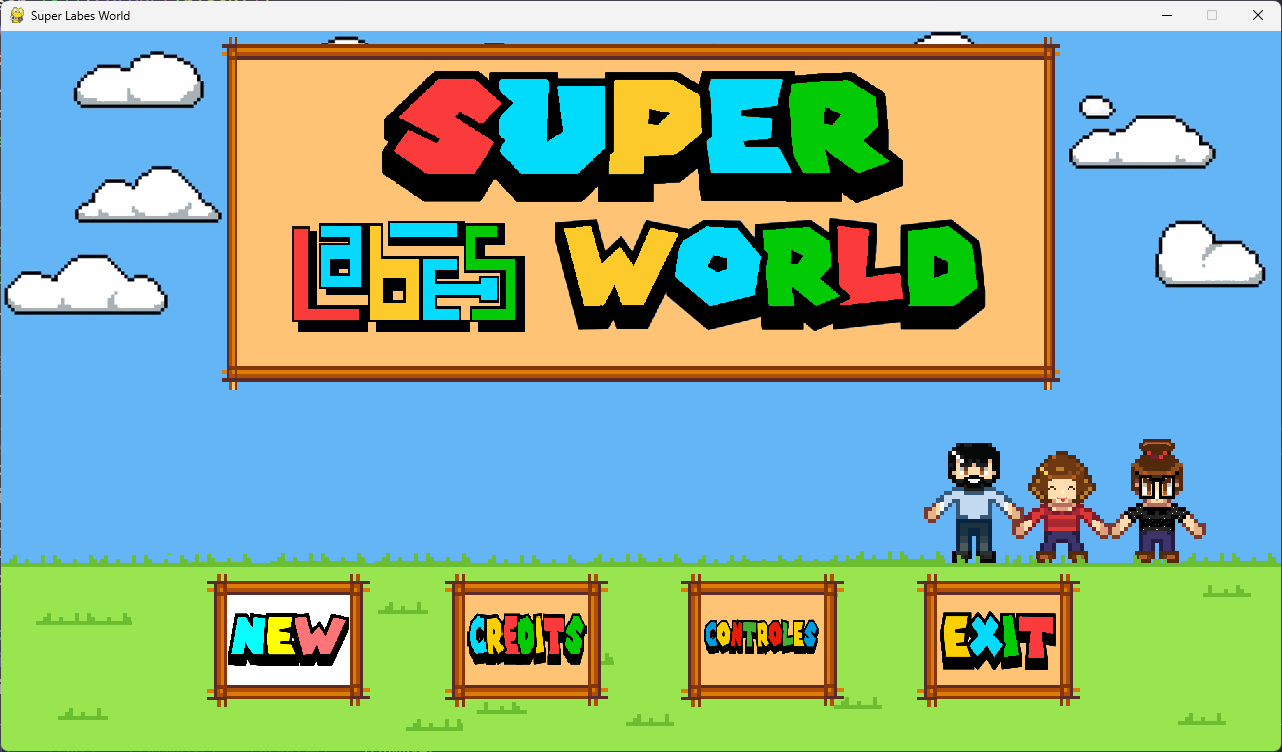
\includegraphics[width=1\linewidth]{figuras/home-super-labes-world.png}
    \caption{Figura ilustrando a home do jogo}
    \label{fig:home-super-labes-world}
\end{figure}

A próxima tela ilustrada na figura \ref{fig:inventory} mostra como é o \textit{layout} da interface de inventário do jogo. nela é possível ver os items que o jogador carrega e a descrição, sendo o limite do inventário 30 items. 
\begin{figure}[t]
    \centering
    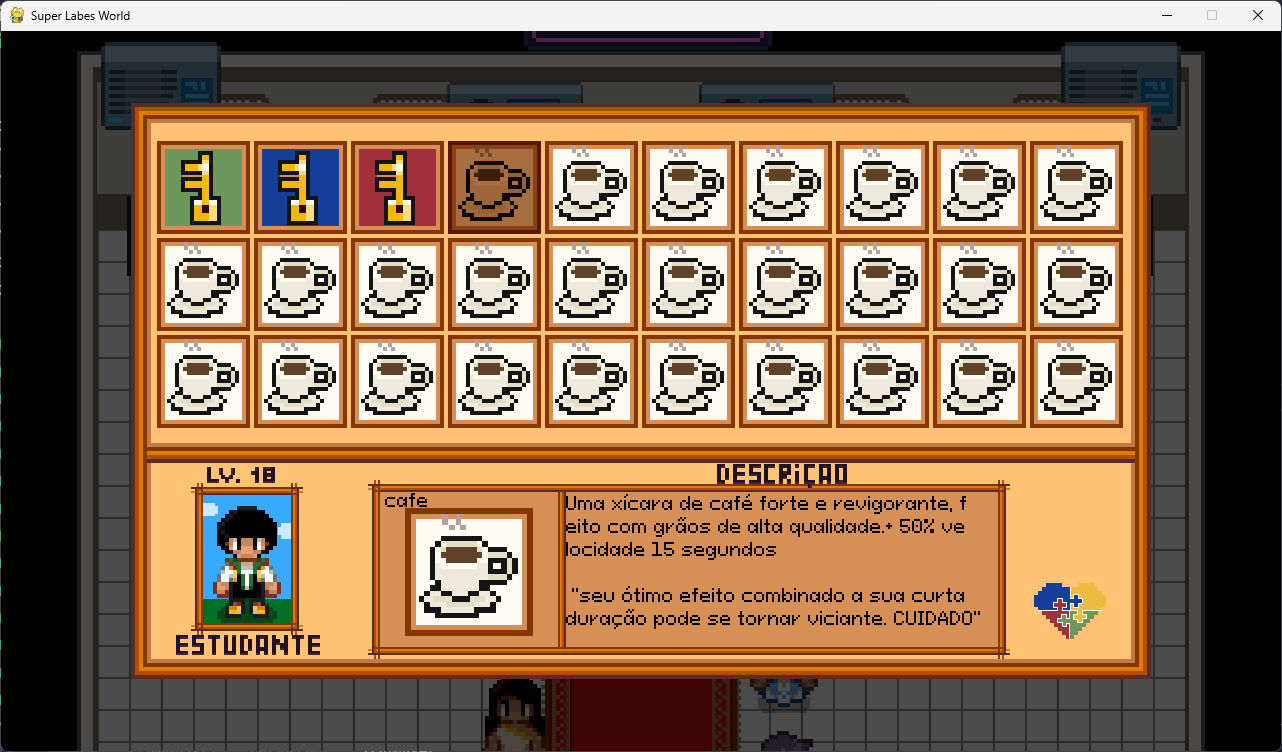
\includegraphics[width=1\linewidth]{figuras/inventory.png}
    \caption{Figura ilustrando o inventário do jogo}
    \label{fig:inventory}
\end{figure}
\clearpage
A figura a seguir \ref{fig:dialog} mostra o jogador interagindo com um dos chefes do jogo na sua sala.

\begin{figure}[h!]
    \centering
    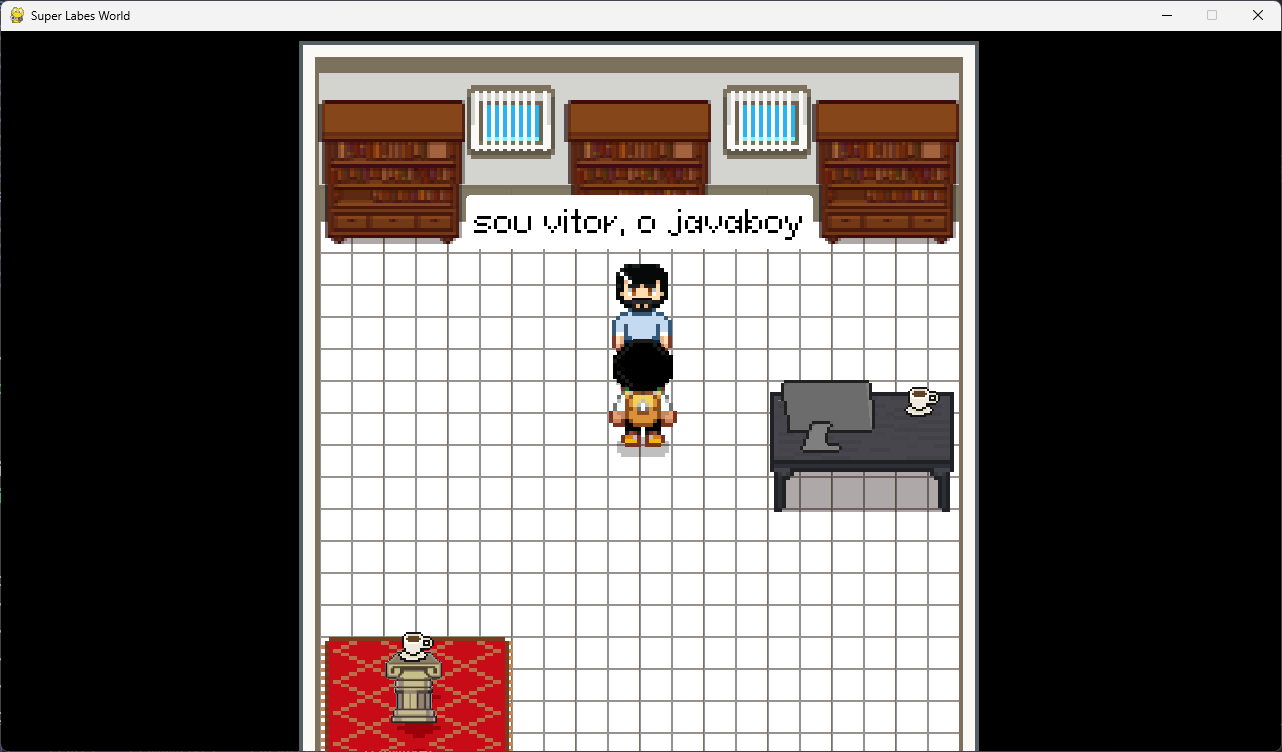
\includegraphics[width=1\linewidth]{figuras/dialog.png}
    \caption{Ilustração de um diálogo do Super Labes World}
    \label{fig:dialog}
\end{figure}
Na figura \ref{fig:battle} podemos ver como é a interface da mecânica principal de jogo a batalha de questões, o retângulo superior esquerdo ilustra a pergunta que o jogador tem que responder, o retângulo superior direito mostra o diálogo feito pelo chefe dependendo da resposta, os retângulos inferiores vermelho, amarelo, verde e azul são a alternativa a ser escolhida pelo jogador cada opção selecionada altera o texto escrito no retângulo inferior esquerdo de cor branca, que é a descrição da resposta. 

\begin{figure}[h!]
    \centering
    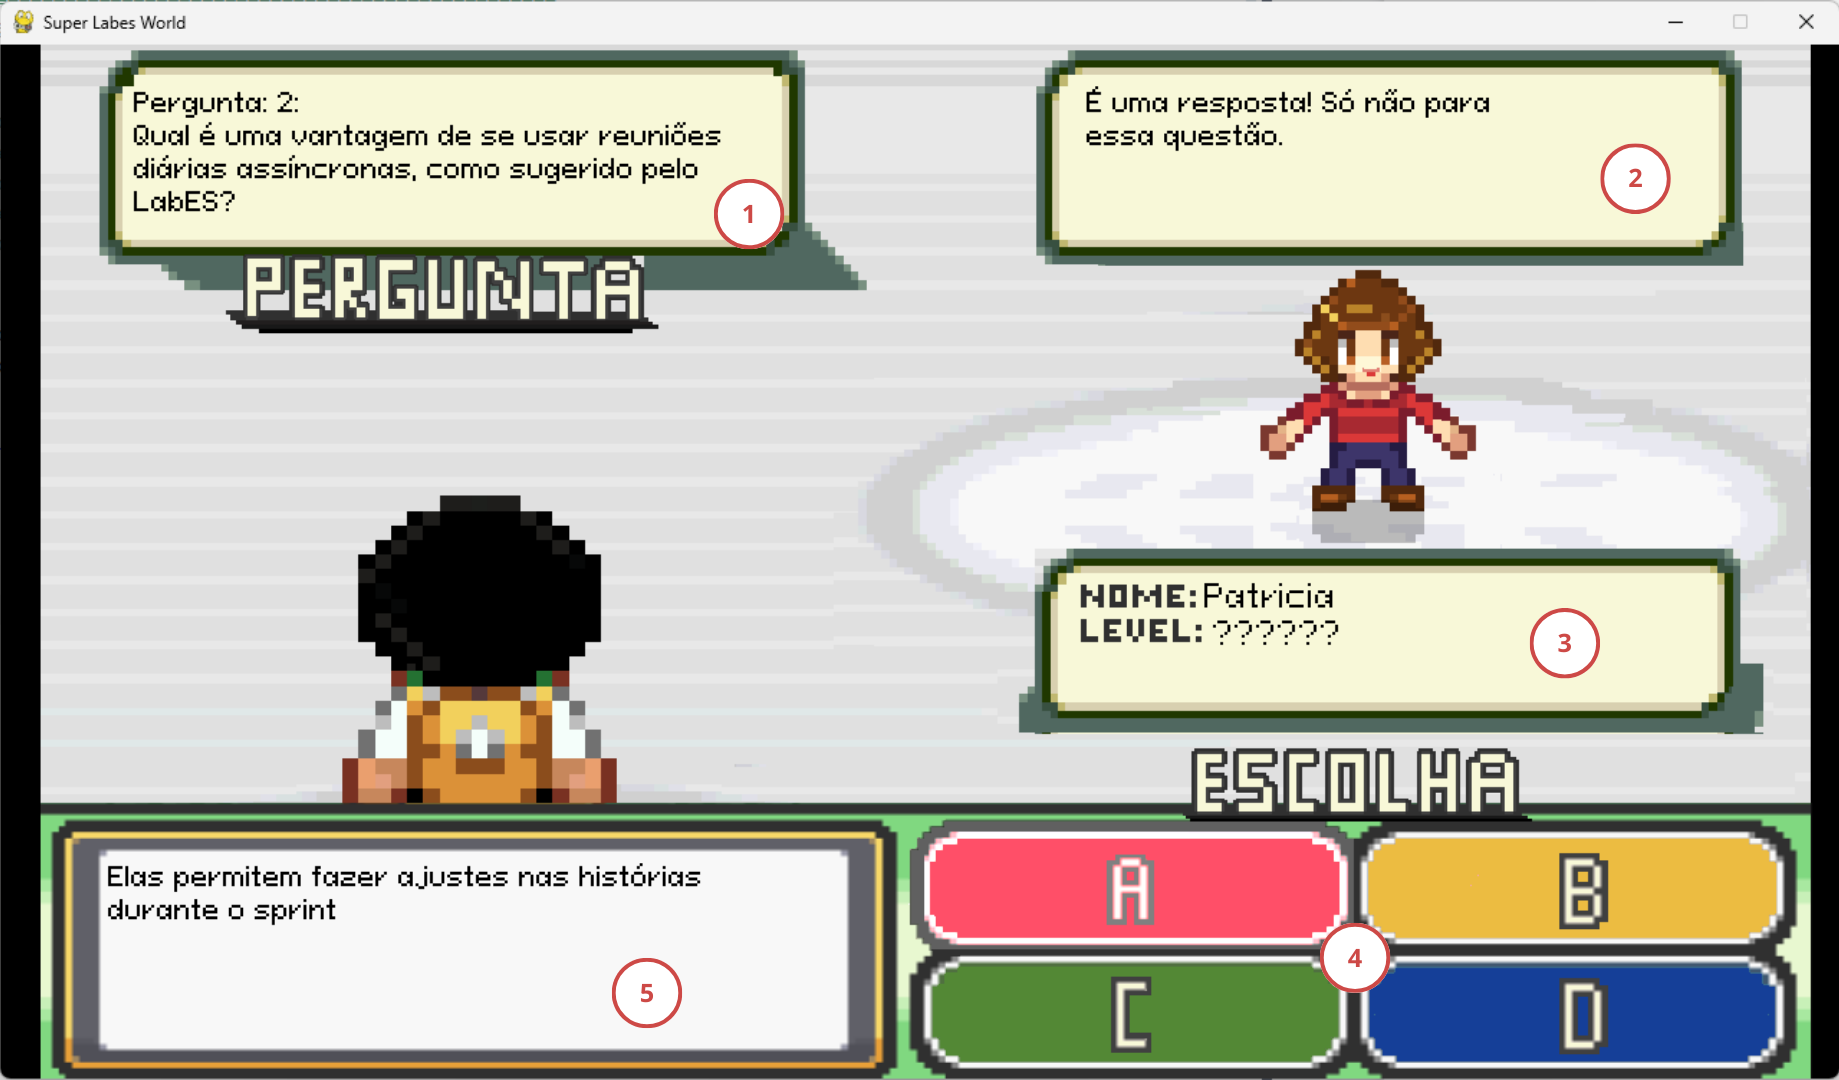
\includegraphics[width=1\linewidth]{figuras/battle.png}
    \caption{Ilustração do sistema de batalha do \textit{game}}
    \label{fig:battle}
\end{figure}